\subsubsection{SSD中采用的损失函数}
\textbf{联合Loss Function:}SSD网络对于每个阶段输出的特征图都进行边框回归和分类操作。SSD网络中作者设计了一个联合损失函数
\begin{equation}
	L(x,c,l,g) = \frac{1}{N}(L_{conf}(x,c) + \alpha L_{loc}(x,l,g)
\end{equation}
其中:

 1、$L_{conf}$表示分类误差,采用多分类的softmax loss
 
 2、$L_{loc}$表示回归误差,采用Smooth L1 loss
 
 3、$\alpha$取1
 
回归loss,smoothL1:
\begin{align}
	L_{loc}(x,l,g) &= \sum _{i \in Pos} ^{N} \sum_{m \in \{cx,cy,w,h\}} x_{ij}^k smooth _{L1} (l_i ^m - g_j ^m) \\
	g_j^{cx} &= \left( g_j ^{cx} - d_i ^{cx} \right) / d_i ^w \quad g_j^{cy} = (g_j^{cy} - d_i^{cy}) / d_i ^h \\
	g_j^w &= \log(\frac{g_j^w}{d_i^w}) \quad g_j^h = \log(\frac{g_j^h}{d_i^h})
\end{align}	
分类误差,采用Softmax Loss:
\begin{equation}
L_{conf}(x, c) = -\sum_{i \in Pos}^N x_{ij}^p\log(c_i^0) \quad where \quad c_i^p = \frac{exp(c_i^p)}{\sum_{p}exp(c_i^p)} 
\end{equation}
\subsubsection{改进损失函数-Focal Loss}
提出Focal Loss的初衷是希望既有”One-Stage Detector“的速度,也有”Two Stage Detector“的准确率。

\textbf{1、为什么"One Stage Detector"的准确率低?}

其作者认为主要原因是:不同类别的训练样本数量的不均衡。在目标检测领域,一张原始图像可能生成非常多的预测区域,但是包含目标的图片数量占比非常低,这就带来了类别不均衡。那么不同类别的训练样本数量不均衡会带来什么后果呢?引用原文讲的两个后果:

(1) training is inefficient as most locations are easy negatives that contribute no useful learning signal; 

(2) en masse, the easy negatives can overwhelm training and lead to degenerate models. \cite{focal-loss}

负样本数量占比过高,使得对总的loss的影响过大,因此使得模型不会按我们所希望的方向进行优化。这也不是新鲜的问题了,先前也有存在一些算法来处理不同类别的训练样本数量不均衡的问题,比如OHEM(Online Hard Example Mining)\cite{ohem},OHEM算法的主要思想可以用原文的一句话概括:In OHEM each example is scored by its loss, non-maximum suppression (NMS\cite{soft-nms}) is then applied, and a minibatch is constructed with the highest-loss examples。\cite{ohem}可以看出OHEM算法加大了对错分类样本的权重,不过OHEM算法忽略了对容易分类的样本的权重处理。Focal Loss是从标准交叉熵损失基础上改进所得。这个函数可以通过调整易分类样本的权重,使得模型在训练时对难分类的样本更专注。

\textbf{标准交叉熵损失函数}

没有经过加权的分类损失是各个训练样本交叉熵的和,如下图所示:

\begin{equation}
CE(p,y)=\left\{
\begin{aligned}
& -\log (p) 	&if y = 1\\
& -\log (1-p) 	&otherwise
\end{aligned}
\right.
\end{equation}

其中:

CE表示cross entropy,p表示预测样本属于1的概率,y表示label,y的取值为{+1,-1},这里仅仅以二分类为例,多分类以此类推。为了表示简便,我们用$p_t$表示样本属于true class的概率。所以上式可以写成

\begin{equation}
	CE(p,y) = CE(p_t) = -\log (p_t)	
\end{equation}
	
\textbf{平衡交叉熵}

我们知道了"One Stage Detector"在训练的时候正负样本的数量差距很大,那么一种常见的做法就是给正负样本加上权重,负样本出现的频次多,那么就降低负样本的权重,正样本数量少,就相对提高正样本的权重,如下式所示:
\begin{equation}
	CE(p_t) = -\alpha \log (p_t)
\end{equation}
	
\textbf{Focal-Loss定义}

通过上述分析,此文作者解决了easy example与hard example数量不均衡的问题,Focal Loss相当于是对各个样本根据网络模型预测该样本属于真实类别的概率设置各自的权重,如果网络对该样本属于真实类别的预测后的概率很大,那么这个样本就属于easy example,相反,对这个网络来说该样本就属于hard example。所以降低绝大部分简单样本的权重,相对增大复杂样本的权重就能训练出一个有效的分类器。Focal Loss的形式如下: 
\begin{equation}
	FL(p_t) = -(1 - p_t)^\gamma \log (p_t)
\end{equation}
参数$\gamma > 0$。当参数$\gamma = 0$的时候,就是普通的交叉熵,作者经过实验发现当$\gamma = 2$时效果最好。从公式中可以发现,当$\gamma
$是一个定值时,比如说等于2,简单样本($p_t = 0.9$)的loss要比标准的交叉熵计算出的loss小100多倍,当$p_t=0.968$时,要小1000多倍,对于困难样本($p_t < 0.5$),loss最多小了4倍。这样的话困难样本的权重相对就提升了很多。 
\begin{equation}
	FL(p_t) = -\alpha _t(1 - p_t)^\gamma \log (p_t)
\end{equation}

\subsubsection{改进NMS,采用Soft-NMS}
本设计中使用到了NMS-非极大值抑制\cite{nms}进行后处理。NMS通常的做法是将检测框按得分排序,然后保留得分最高的框,同时删除与该框重叠面积大于一定比例的其它框。这种贪心式方法存在如图所示的问题: 
\begin{uscfigure}
	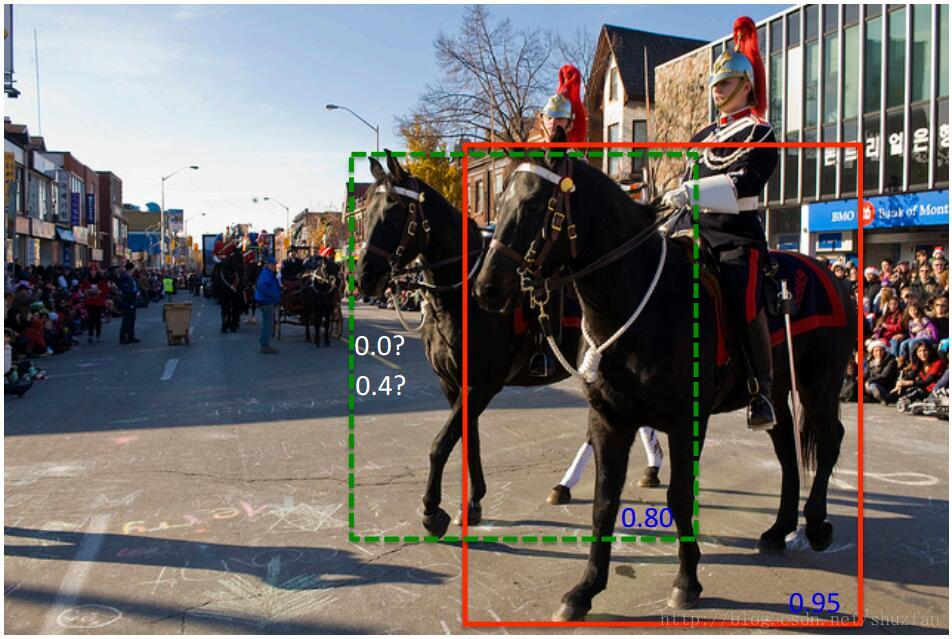
\includegraphics[width=\textwidth]{./Pictures/soft-nms.jpeg}	
	\caption{非极大值抑制}
	\label{soft-nms}
\end{uscfigure}
红色框和绿色框是当前的检测结果,二者的得分分别是0.95和0.80。如果按照传统的NMS进行处理,首先选中得分最高的红色框,然后绿色框就会因为与之重叠面积过大而被删掉。另一方面,NMS的阈值也不太容易确定,设小了会出现下图的情况(绿色框因为和红色框重叠面积较大而被删掉),设置过高又容易增大误检。

Soft-NMS采用的策略是用降低置信度来取代直接删除掉IOU大于阈值的框。原来的NMS可以描述如下:
\begin{equation}
s_i=\left\{
\begin{aligned}
& s_i 	&iou(M,b_i) < N_t,\\
& 0 	&otherwise
\end{aligned}
\right.
\end{equation}
现在我们将其替换成如下形式:
\begin{equation}
s_i=\left\{
\begin{aligned}
& s_i 	&iou(M, b_i) < N_t\\
& s_i(1 - iou(M, b_i)) 	&otherwise
\end{aligned}
\right.
\end{equation}